In this chapter the client and it's functions are described. The Client exists of the following subsystems:
\begin{shortlist}
    \item MQTT
    \item Message/Config Parser
    \item Audio driver
    \item Relative Weight Factor
    \item Logger
\end{shortlist}

The aforementioned parts will be described in the following sections.

\section{MQTT}

The client uses the \href{http://mosquitto.org/}{Mosquitto MQTT C++ library}.
This is an open source message broker that implements the MQTT protocol versions 3.1 and 3.1.1.
MQTT is a publish-subscribe based \say{light weight} messaging protocol for use on top of the TCP/IP protocol.
It is designed for connections with remote locations where a \say{small code footprint} is required or the network bandwidth is limited.
This makes it suitable for \say{Internet of Things} messaging.

The client and the website use topics to communicate. The topics for the communication are described in the previous chapter.
The DNS class has a public inheritance of the Mosquito class.
This means all public and protected members of the Mosquitto class can be accessed by the DNS class.
The private members cannot directly accessed by DNS class. In the DNS class the Mosquitto functions are been overwritten by DNS's own implementation.
The Mosquitto functions are automatically called by the Mosquitto library.

If the client is executed the Mosquitto library calls the function
\textbf{ on connect}. This function published the client-id in the \textbf{online topic } and subscribe itself on the following topics:
\small{
\begin{itemize} [noitemsep, nolistsep]
	\item \textbf {request online}
	\item \textbf {request client data}
	\item \textbf {clients data}
	\item \textbf {music volume}
	\item \textbf {music status}
	\item \textbf {music sources}
\end{itemize}
}

If the client is stopped or disconnected the Mosquitto library calls the function \textbf {on disconnect}. This function published the client-id in the \textbf {offline topic}.\\

When the client is running and has excuted the function \textbf {on connect}. He waits on a message from a subscribed topic. If there appears a message, the function \textbf {on message} is called. This function has as parameters a mosquitto message struct. This contains:
\small{
\begin{itemize} [noitemsep, nolistsep]
	\item \textbf {int mid}
	\item \textbf {char *topic}
	\item \textbf {void* payload}
	\item \textbf {int payloadlen}
	\item \textbf {int qos}
	\item \textbf {bool retain\\}
\end{itemize}
}

In the function is watched on which topic a message is send. This is done by compare the \textbf {char *topic} of the mosquitto message struct with the defined topic described in chapter 2. When there is a match, a action is carried out.\\

MQTT has a funcion that is called \textbf {last will}. This function is called when a client abruptly disconnected and published his last will message. This can means that the client crashed, hasn't a connection to the broker or something else. In the client this function is implemented and the client will publish his message to the \textbf {offline} topic.

\section{Message/Config Parser}

Almost all the messages that are been send in this application are in \href{http://www.json.org/}{JSON string format}. In C++ this is a bit difficult because the native language doesn't include a JSON Parser. In the client the \href{https://github.com/Zguy/Jzon}{library JZON} is used to parse the JSON string formats.\\

The client must be provided with a file with data in JSON format to be used to initialize the client. The data that can be specified is:
\small{
\begin{itemize} [noitemsep, nolistsep]
	\item \textbf {Names}
	\item \textbf {Log info}
	\item \textbf {Prefixs}
	\item \textbf {Brokers}
	\item \textbf {Topics\\}
\end{itemize}
}
With this it's possible to define the data mentioned above in the config file and it can be used to initialize the clients and the website. The benefits of doing this is that you only have to change the config file and everything still works instead of changing every client individually.

\\section{Audio driver}
\label{sec:client_audio_driver}
Audio driver

\section{Relative Weight Factor}
\label{sec:client_relative_weight_factor}

This system is based on a virtual object that will create sound like it is in some place in 2D space.
This library calculates the volume level that a speaker needs to be in comparison with all the other speakers.

\subsection{The problem}
\label{sub:client_rwf_the_problem}

The explain the inner workings lets look at an example.

In figure \ref{fig:client_rwf_center} is a simple setup. Two speakers, a virtual object that \say{creates} the sound and the real life user that listens to this.
The speakers are the actual devices that are creating the sound.
What the goal of these speaker is, is to reenact the sound that comes out of a speaker at such a sound level that the user is thinking that the sound comes from a certain place.
In the aforementioned figure, it is clear that the sound levels need to be of the same volume.
That way, the user thinks that the sound at that place is equally as loud, so it is the center of the volume.
\begin{figure}[H]
    \centering
    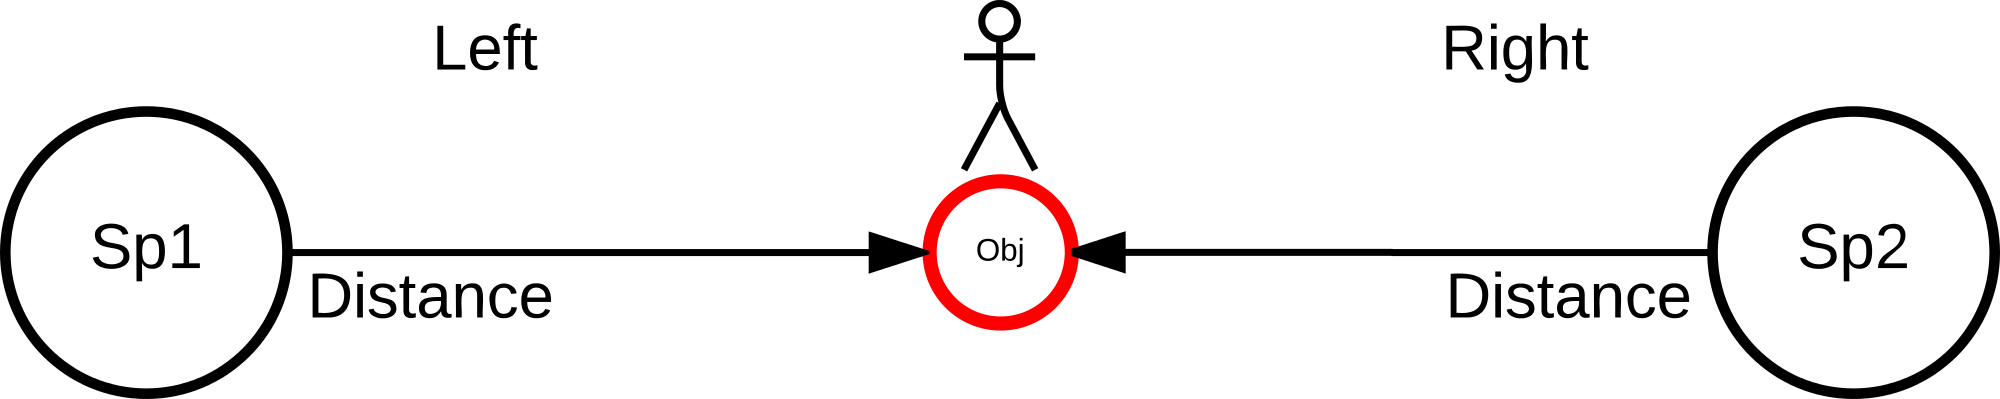
\includegraphics[width=.8\textwidth]{client_rwf_center}
    \caption{Virtual object at center}
    \label{fig:client_rwf_center}
\end{figure}

In figure \ref{fig:client_rwf_offset} is the next example. Now the virtual object is at an offset from the user.
you would normally say that \say{Sp1} has a shorter distance and \say{Sp2} has a greater distance.
To compensate, \say{Sp2} needs to be harder then \say{Sp1}. Let's think about this for a minute.
If the user is standing in the middle and \say{Sp2} is playing harder then \say{Sp1}.
This means that the \say{Right} side produces more sound then the \say{Left} side.
The user would hear more sound comming from the \say{Right} side, so the user would think that the sound comes from the \say{Right} side.

\begin{figure}[H]
    \centering
    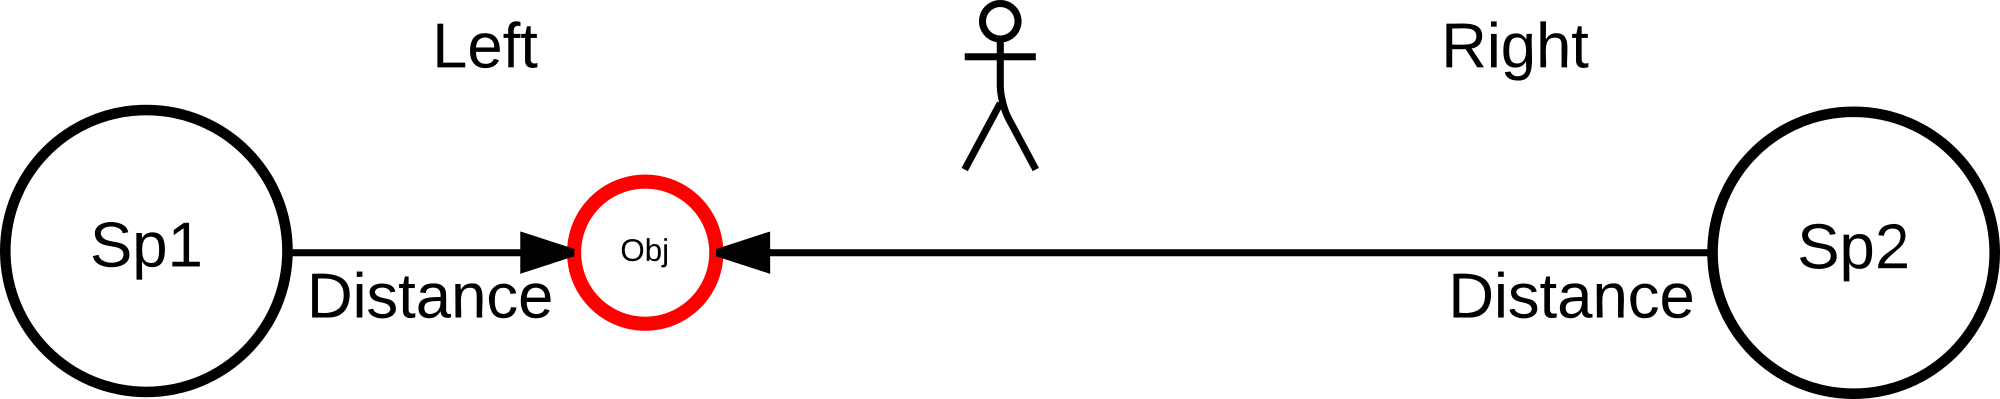
\includegraphics[width=.8\textwidth]{client_rwf_offset}
    \caption{Virtual object at offset}
    \label{fig:client_rwf_offset}
\end{figure}

In conclusion the speaker where the object is closed to, needs to produce the most sound.

\subsection{Calculating value}
\label{sub:client_rwf_calculating_value}

\begin{spreadtab}{{tabular}{ l | r || r l l | r l l }}
    @Speaker    & @Distance                         & @\multicolumn{3}{c|}{Inverse distance}& @\multicolumn{3}{c}{Calculated Value} \\
    @A          & 1                                 & :={b5}&-:={b2}&= :={b5-b2}            &  :={e2}&*:={e10}&= :={round(e2*(e9/e5), 0)} \\
    @B          & 2                                 & :={b5}&-:={b3}&= :={b5-b3}            &  :={e3}&*:={e10}&= :={round(e3*(e9/e5), 0)}\\
    @C          & 3                                 & :={b5}&-:={b4}&= :={b5-b4}            &  :={e4}&*:={e10}&= :={round(e4*(e9/e5), 0)}\\
    @Total:     & sum(b2:b4)                        &       &       &= :={sum(e2:e4)}       &  \\ \hline
                &                                   &       &       &                       &  \\
    @\multicolumn{2}{r ||}{Head}                    & 100   &       &                       &  \\
    @\multicolumn{2}{r || }{Tail}                   & 0     &       &                       &  \\
    @\multicolumn{2}{r || }{Volume steps}           & :={c7}&-:={c8}& = :={c7-c8}           & \\
    @\multicolumn{2}{r || }{Value per volume step}  & :={e9}&/:={e5}& = :={round(e9/e5, 2)} & \\
\end{spreadtab}

\section{Logger}
\label{sec:client_logger}
Logger
